\documentclass[11pt]{article}
\usepackage{graphicx}
\usepackage{url}

\title{GitHub for Mathematical Research}
\author{Luke Guatelli and Andrew Penland}
\date{\today}

\begin{document}

\maketitle

\section{Introduction to GitHub}

\subsection{Overview}

\textit{Git} is a version control system - a piece of software that can be used to track changes and other information about projects. \textit{GitHub} is an online platform that uses Git. GitHub is widely used by software developers, and it contains a \textit{lot} of open source software. It is a standard tool in the software industry. 

\subsection{Why Use GitHub?}

It makes editing and version control easier. -AP

\section{How To Do Specific Things}

\subsection{Create An Account}

\subsection{Start a Project}

\subsection{Add a File}

\subsection{Invite a Collaborator} 

\url{https://github.community/t5/How-to-use-Git-and-GitHub/Where-do-I-see-all-incoming-invitations-collaborator/td-p/4280}

\subsection{Manage Issues}

Issues are a way for team members to communicate and keep track of changes to the project.  Here is GitHub's description of an issue:~\cite{github-issues} \\

\begin{quote}
Issues are used to track todos, bugs, feature requests, and more. As issues are created, they'll appear here in a searchable and filterable list. To get started, you should \underline{create an issue.}
\end{quote} 

\subsubsection{Creating An Issue}
We'll follow their advice, creating our first issue. The first issue we will create will be a ``\texttt{todo}'', telling us to create an issue. (Thus, this issue resolves itself.) We have two options: 

\begin{enumerate}

\item Under the 
\includegraphics{PlusMenu} in the upper left corner,we select the command ``New Issue''. \\

\begin{center}
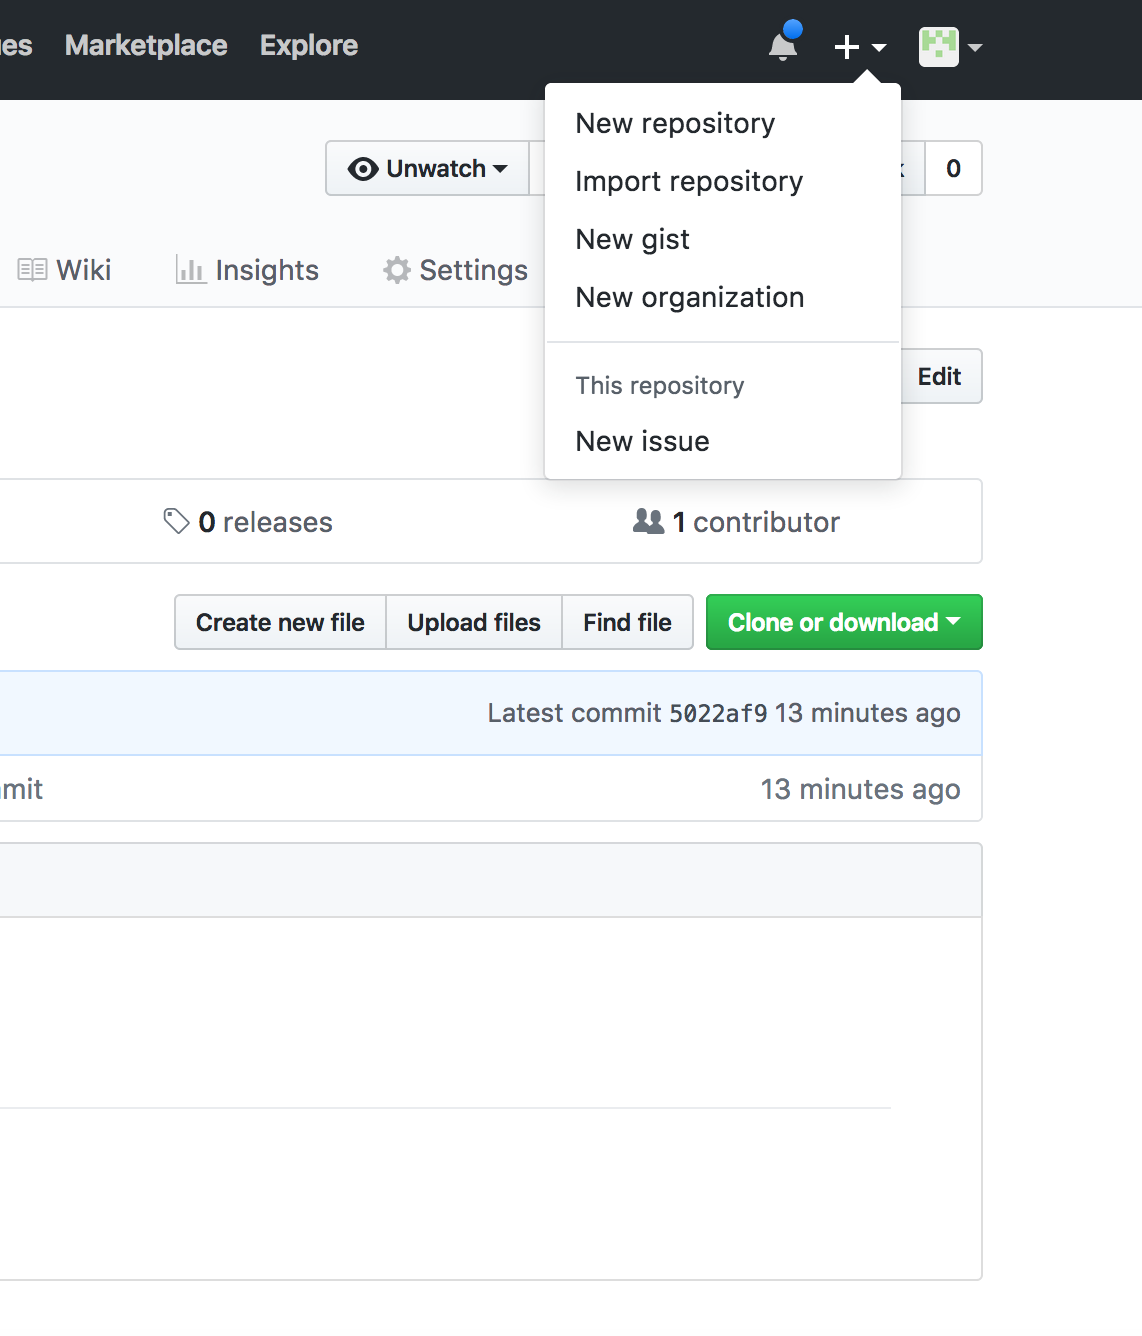
\includegraphics[width=0.5\textwidth]{NewIssueMenu}
\end{center}

\item We click on the 
\includegraphics[width=0.75in]{IssuesLink} tab, then click the 
\includegraphics[width=0.75in]{NewIssueButton} button. 

\end{enumerate} 

Either way brings up a ``New Issue'' screen with fields for Title and Description. We fill in this information, then click the 
\includegraphics[width=0.75in]{SubmitNewIssue} button. 

\begin{center}
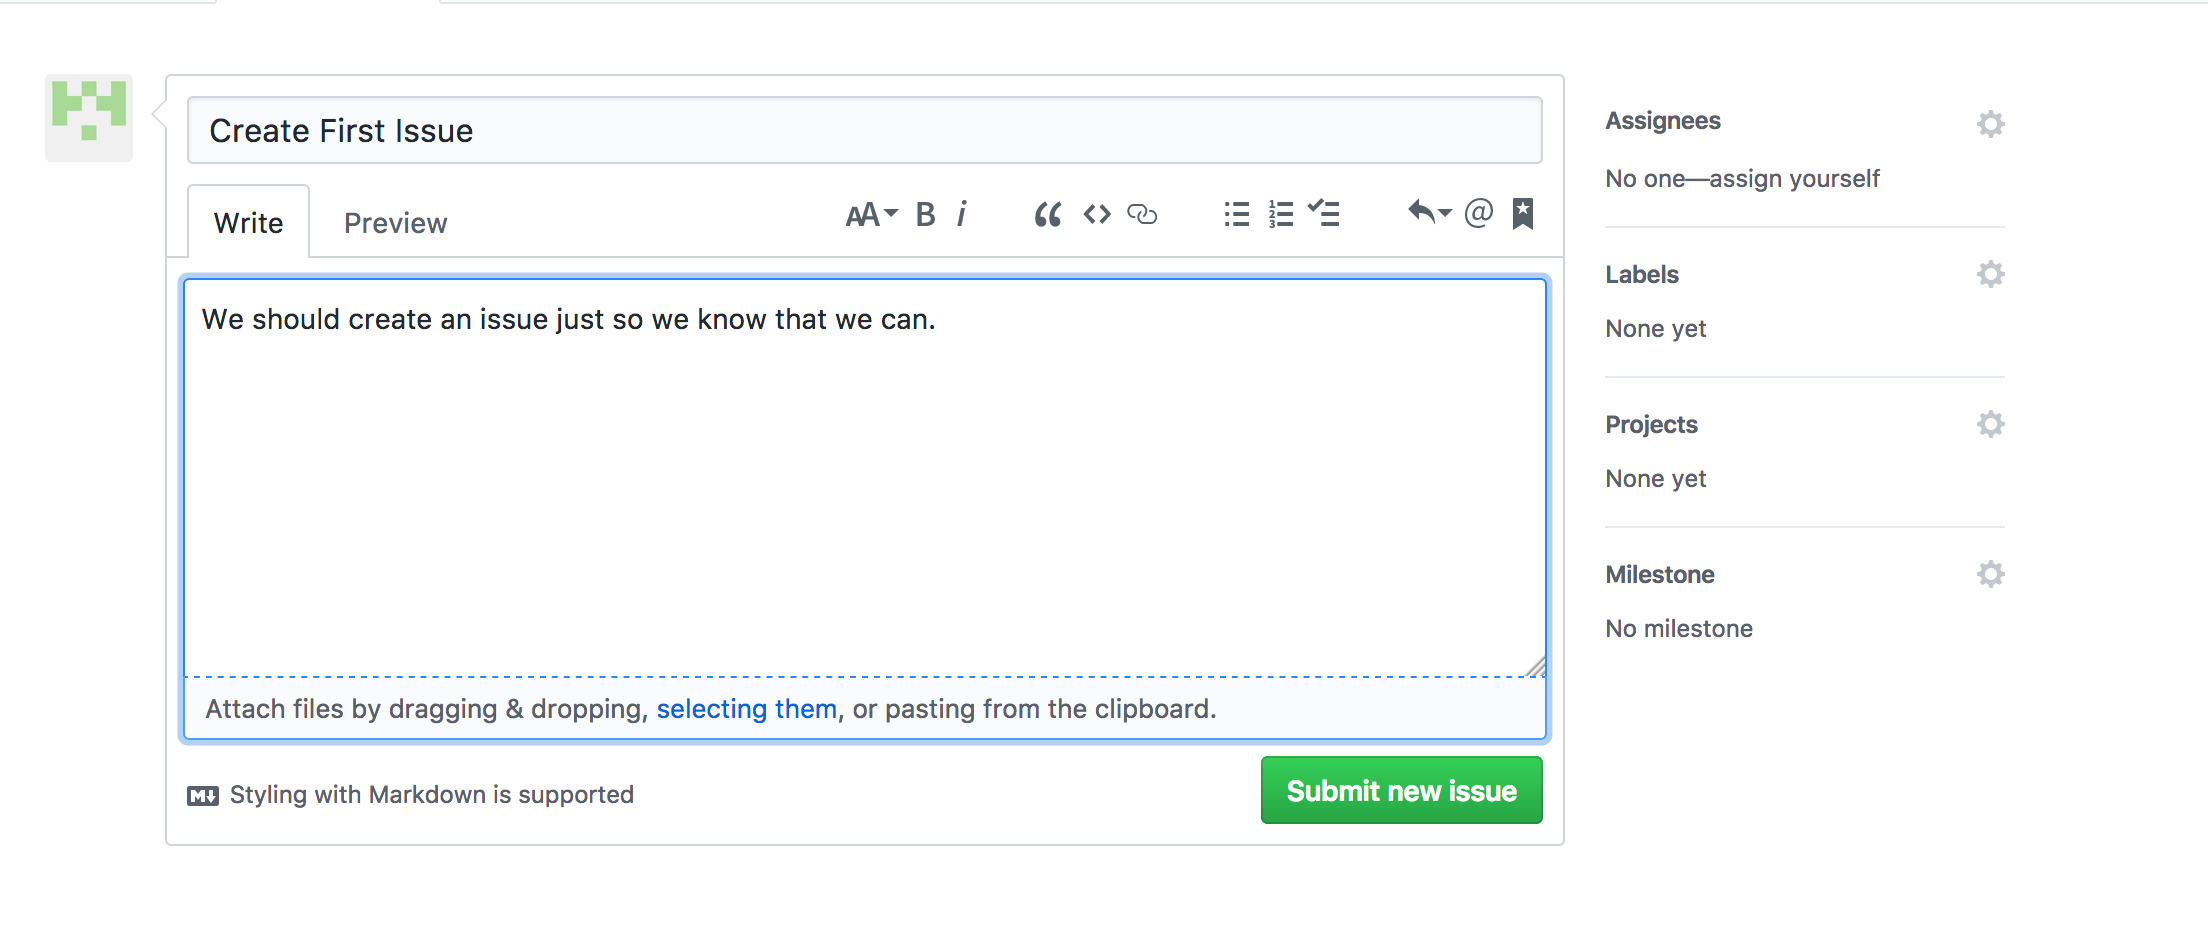
\includegraphics[width=\textwidth]{CreatingAnIssue}
\end{center}

\subsubsection{Checking For Issues}

If we log in to GitHub, we see that there is a new Issue by checking the ``Issues'' tab. We see 
\includegraphics[width=0.75in]{IssuesLink}, telling us there is one new issue. We click on the tab to see what the issue is.

\subsubsection{Closing An Issue} 

Once an issue is satisfactorily resolved, we want to close it. We can do this on the Issues screen by selecting the checkbox next to the issue, then going to the ``Mark as'' menu and selecting ``Closed''.

\begin{center}
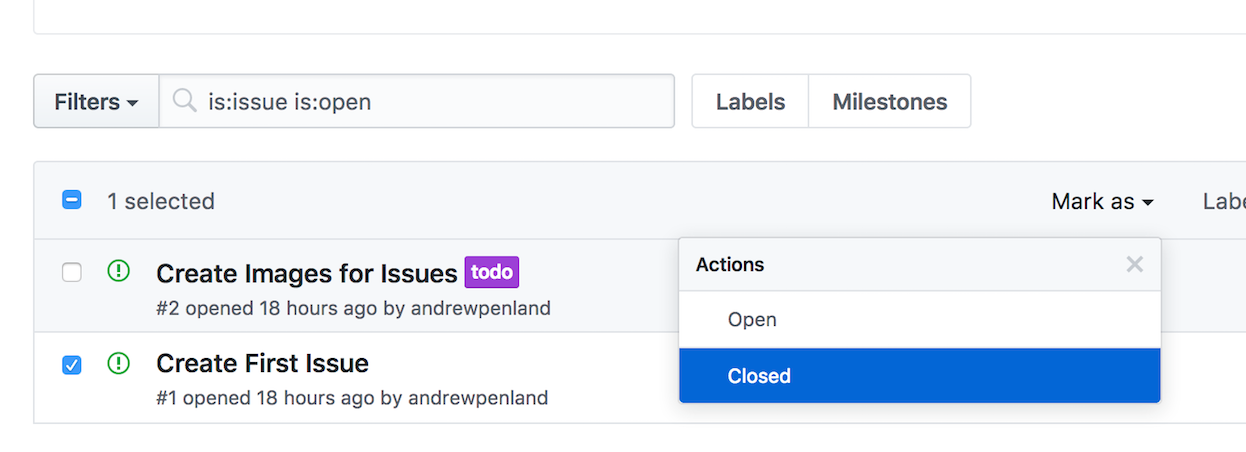
\includegraphics[width=0.9\textwidth]{MarkIssueClosed}
\end{center}

\subsubsection{Labeling Issues}

We can label issues so that we know what type they are. We can label an issue when we create it by using a dropdown menu called ``Labels''. GitHub has pre-existing labels for various categories. Simply type the name of the label you want to use or select it from the menu. 

To create our own label, we begin by typing the name we want to use for the label. GitHub will automatically bring up a suggestion to create a label with this name.

Figure~\ref{fig:begin-typing-todo} and Figure~\ref{fig:todo-label-details} show how to create a ``todo'' label, which is a common issue that doesn't have a premade GitHub label. 


\begin{figure}\label{fig:begin-typing-todo}
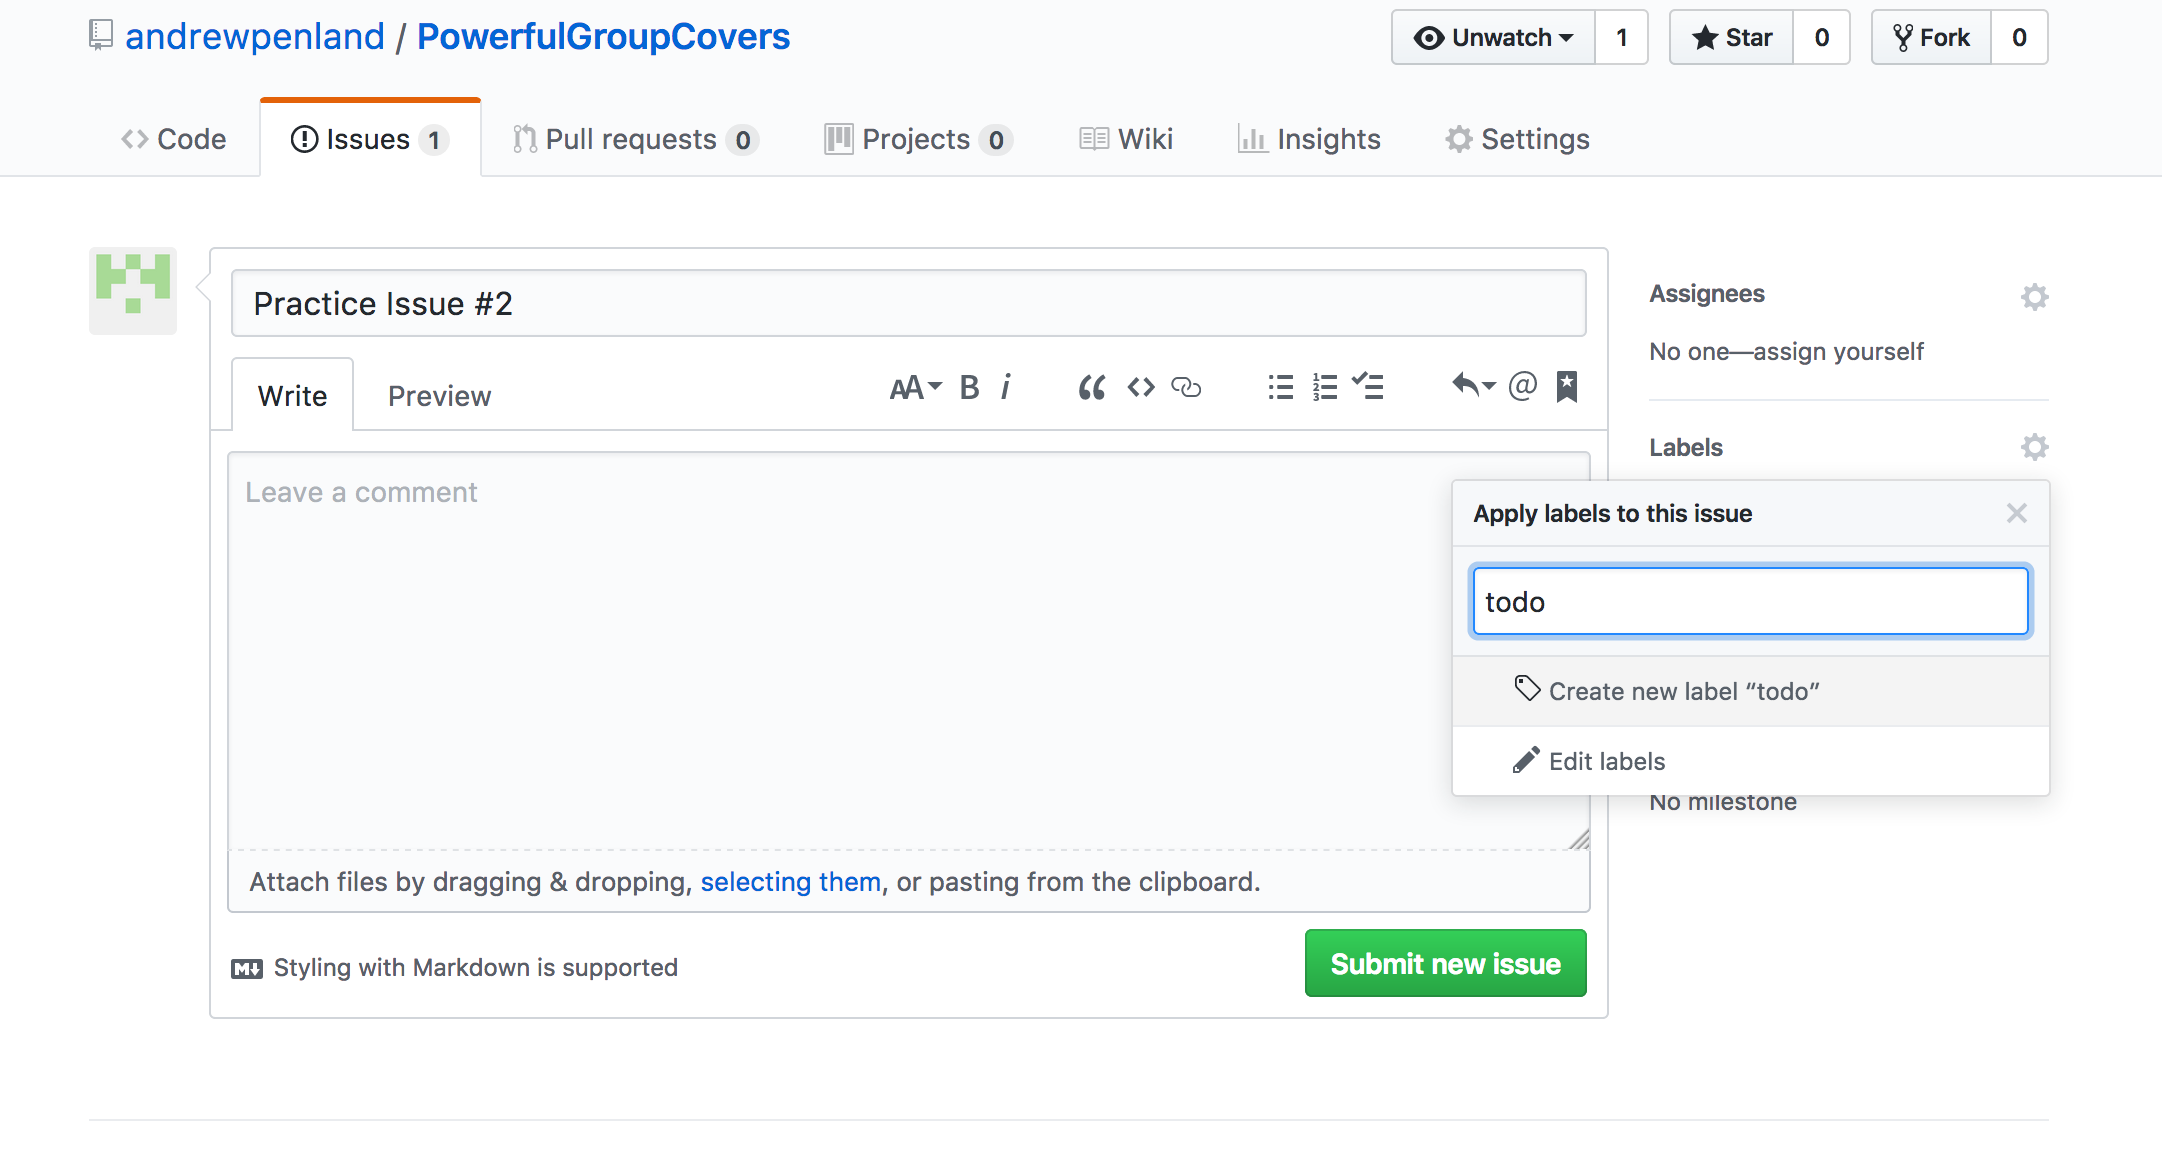
\includegraphics[width=0.9\textwidth]{CreatingLabels}
\caption{Labeling An Issue using The Menu}
\end{figure}

\begin{figure}\label{fig:todo-label-details}
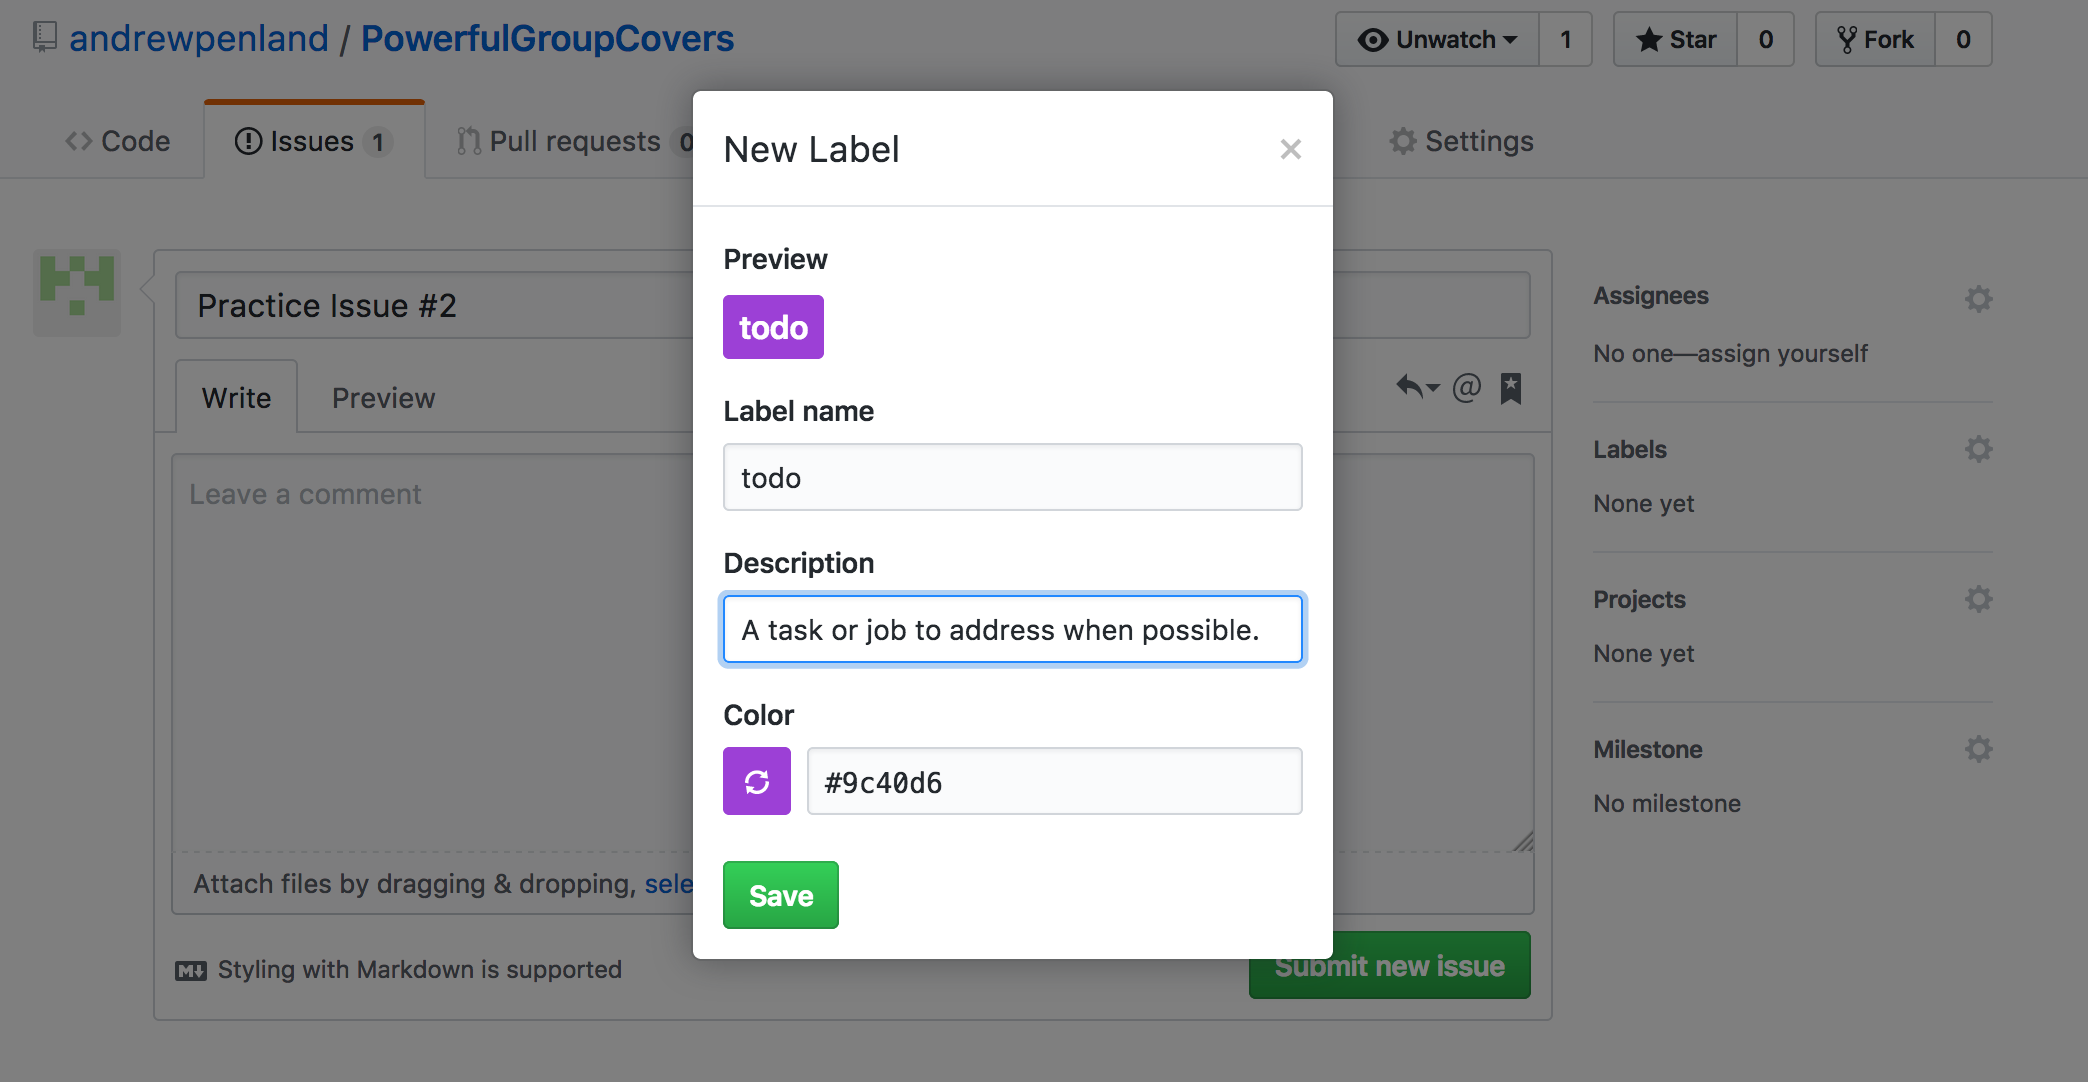
\includegraphics[width=0.9\textwidth]{NewLabelBox}
\caption{Creating A Custom Label}
\end{figure}


\subsubsection{Assigning Issues}

You can assign an issue to the attention of specific project members using the ``Assignments'' drop-down menu, which is to the right of the screen just above the ``Labels'' menu. 

\subsection{Pull Requests}

\subsection{Keeping Track of Changes}

\section{Conclusion}

\end{document}
